%%%%%%%%%%%%%%%%%%%%%%%%%%%%%%%%%%%%%%%%%
% Wenneker Article
% LaTeX Template
% Version 2.0 (28/2/17)
%
% This template was downloaded from:
% http://www.LaTeXTemplates.com
%
% Authors:
% Vel (vel@LaTeXTemplates.com)
% Frits Wenneker
%
% License:
% CC BY-NC-SA 3.0 (http://creativecommons.org/licenses/by-nc-sa/3.0/)
%
%%%%%%%%%%%%%%%%%%%%%%%%%%%%%%%%%%%%%%%%%

%----------------------------------------------------------------------------------------
%	PACKAGES AND OTHER DOCUMENT CONFIGURATIONS
%----------------------------------------------------------------------------------------

\documentclass[10pt, a4paper, twocolumn]{article} % 10pt font size (11 and 12 also possible), A4 paper (letterpaper for US letter) and two column layout (remove for one column)

%%%%%%%%%%%%%%%%%%%%%%%%%%%%%%%%%%%%%%%%%
% Wenneker Article
% Structure Specification File
% Version 1.0 (28/2/17)
%
% This file originates from:
% http://www.LaTeXTemplates.com
%
% Authors:
% Frits Wenneker
% Vel (vel@LaTeXTemplates.com)
%
% License:
% CC BY-NC-SA 3.0 (http://creativecommons.org/licenses/by-nc-sa/3.0/)
%
%%%%%%%%%%%%%%%%%%%%%%%%%%%%%%%%%%%%%%%%%

%----------------------------------------------------------------------------------------
%	PACKAGES AND OTHER DOCUMENT CONFIGURATIONS
%----------------------------------------------------------------------------------------

\usepackage[english]{babel} % English language hyphenation

\usepackage{microtype} % Better typography

\usepackage{amsmath,amsfonts,amsthm} % Math packages for equations

\usepackage[svgnames]{xcolor} % Enabling colors by their 'svgnames'

\usepackage[hang, small, labelfont=bf, up, textfont=it]{caption} % Custom captions under/above tables and figures

\usepackage{booktabs} % Horizontal rules in tables

\usepackage{lastpage} % Used to determine the number of pages in the document (for "Page X of Total")

\usepackage{graphicx} % Required for adding images

\usepackage{placeins} % For FloatBarrier

\usepackage{enumitem} % Required for customising lists
\setlist{noitemsep} % Remove spacing between bullet/numbered list elements

\usepackage{sectsty} % Enables custom section titles
\allsectionsfont{\usefont{OT1}{phv}{b}{n}} % Change the font of all section commands (Helvetica)

%----------------------------------------------------------------------------------------
%	MARGINS AND SPACING
%----------------------------------------------------------------------------------------

\usepackage{geometry} % Required for adjusting page dimensions

\geometry{
	top=1cm, % Top margin
	bottom=1.5cm, % Bottom margin
	left=2cm, % Left margin
	right=2cm, % Right margin
	includehead, % Include space for a header
	includefoot, % Include space for a footer
	%showframe, % Uncomment to show how the type block is set on the page
}

\setlength{\columnsep}{7mm} % Column separation width

%----------------------------------------------------------------------------------------
%	FONTS
%----------------------------------------------------------------------------------------

\usepackage[T1]{fontenc} % Output font encoding for international characters
\usepackage[utf8]{inputenc} % Required for inputting international characters

\usepackage{XCharter} % Use the XCharter font

%----------------------------------------------------------------------------------------
%	HEADERS AND FOOTERS
%----------------------------------------------------------------------------------------

\usepackage{fancyhdr} % Needed to define custom headers/footers
\pagestyle{fancy} % Enables the custom headers/footers

\renewcommand{\headrulewidth}{0.0pt} % No header rule
\renewcommand{\footrulewidth}{0.4pt} % Thin footer rule

\renewcommand{\sectionmark}[1]{\markboth{#1}{}} % Removes the section number from the header when \leftmark is used

%\nouppercase\leftmark % Add this to one of the lines below if you want a section title in the header/footer

% Headers
\lhead{} % Left header
\chead{\textit{\thetitle}} % Center header - currently printing the article title
\rhead{} % Right header

% Footers
\lfoot{} % Left footer
\cfoot{} % Center footer
\rfoot{\footnotesize Page \thepage\ of \pageref{LastPage}} % Right footer, "Page 1 of 2"

\fancypagestyle{firstpage}{ % Page style for the first page with the title
	\fancyhf{}
	\renewcommand{\footrulewidth}{0pt} % Suppress footer rule
}

%----------------------------------------------------------------------------------------
%	TITLE SECTION
%----------------------------------------------------------------------------------------

\newcommand{\authorstyle}[1]{{\large\usefont{OT1}{phv}{b}{n}\color{DarkRed}#1}} % Authors style (Helvetica)

\newcommand{\institution}[1]{{\footnotesize\usefont{OT1}{phv}{m}{sl}\color{Black}#1}} % Institutions style (Helvetica)

\usepackage{titling} % Allows custom title configuration

\newcommand{\HorRule}{\color{DarkGoldenrod}\rule{\linewidth}{1pt}} % Defines the gold horizontal rule around the title

\pretitle{
	\vspace{-30pt} % Move the entire title section up
	\HorRule\vspace{10pt} % Horizontal rule before the title
	\fontsize{20}{24}\usefont{OT1}{phv}{b}{n}\selectfont % Helvetica
	\color{DarkRed} % Text colour for the title and author(s)
}

\posttitle{\par\vskip 15pt} % Whitespace under the title

\preauthor{} % Anything that will appear before \author is printed

\postauthor{ % Anything that will appear after \author is printed
	\vspace{10pt} % Space before the rule
	\par\HorRule % Horizontal rule after the title
	\vspace{20pt} % Space after the title section
}

%----------------------------------------------------------------------------------------
%	ABSTRACT
%----------------------------------------------------------------------------------------

\usepackage{lettrine} % Package to accentuate the first letter of the text (lettrine)
\usepackage{fix-cm}	% Fixes the height of the lettrine

\newcommand{\initial}[1]{ % Defines the command and style for the lettrine
	\lettrine[lines=3,findent=4pt,nindent=0pt]{% Lettrine takes up 3 lines, the text to the right of it is indented 4pt and further indenting of lines 2+ is stopped
		\color{DarkGoldenrod}% Lettrine colour
		{#1}% The letter
	}{}%
}

\usepackage{xstring} % Required for string manipulation

\newcommand{\lettrineabstract}[1]{
	\StrLeft{#1}{1}[\firstletter] % Capture the first letter of the abstract for the lettrine
	\initial{\firstletter}\textbf{\StrGobbleLeft{#1}{1}} % Print the abstract with the first letter as a lettrine and the rest in bold
}

%----------------------------------------------------------------------------------------
%	BIBLIOGRAPHY
%----------------------------------------------------------------------------------------

\usepackage[backend=bibtex,style=authoryear,natbib=true]{biblatex} % Use the bibtex backend with the authoryear citation style (which resembles APA)

\addbibresource{example.bib} % The filename of the bibliography

\usepackage[autostyle=true]{csquotes} % Required to generate language-dependent quotes in the bibliography
 % Specifies the document structure and loads requires packages

%----------------------------------------------------------------------------------------
%	ARTICLE INFORMATION
%----------------------------------------------------------------------------------------

\title{Sollten Algorithmen im Gericht benutzt werden, um die Rückfälligkeitswahrscheinlichkeit von Angeklagten zu berechnen? } % The article title

\author{
	\authorstyle{Gruppe: 10\\ Journalist: Jonas Opitz\\ Chefredakteur: Frank Eric Mbouga} % Authors
}

% Example of a one line author/institution relationship
%\author{\newauthor{John Marston} \newinstitution{Universidad Nacional Autónoma de México, Mexico City, Mexico}}

\date{\today} % Add a date here if you would like one to appear underneath the title block, use \today for the current date, leave empty for no date

%----------------------------------------------------------------------------------------

\begin{document}

\maketitle % Print the title

\thispagestyle{firstpage} % Apply the page style for the first page (no headers and footers)


% -------------------------------------------------------------------------------------------------------------------------------
\section{Einleitung}
Welche Folgen kann es für wen geben, wenn man einen Algorithmus zum Bestimmen der Rückfälligkeitswahrscheinlichkeit von Angeklagten, wie OCEAN, im Gericht einführt?

Nachdem es im vorherigen Blogeintrag darum ging, wie Algorithmen wie Northpointes OCEAN funktionieren, soll es nun um die Konsequenzen der Einführung dieser gehen.

Um diese Frage zu betrachten wird zunächst das soziale System, d.h. die betroffenen Akteure, betrachtet, in das diese Algorithmen eingefügt werden, und ob es sich hier nach Kienle und Kunau um ein sozio-technisches System handelt.
Danach wird noch ein Mal auf die Funktionsweise von OCEAN eingegangen und diskutiert, woher die in [1] beschriebenen rassistischen Tendenzen her kommen könnten.
Zuletzt wird die primäre These dieser Diskussion über ein Vestersches Wirkungsgefüge gekräftigt.

Da Algorithmen zum Bestimmen der Rückfälligkeitswahrscheinlichkeit bereits in den USA angewandt werden, und sich die meisten Studien auf die USA beziehen, wird sich dieser Blogeintrag ebenfalls auf die USA beziehen.

% -------------------------------------------------------------------------------------------------------------------------------
\section{Das interagierende soziale System}
Auf erstem Blick scheint es vier Akteure zu geben, die von Algorithmen wie OCEAN betroffen sind:
\begin{itemize}
  \item Die Privatunternehmen, die solche Algorithmen entwickeln, vermieten und somit von ihnen profitieren.
  \item Der Gesetzgeber, der gegebenenfalls den Einsatz dieser Algorithmen regulieren muss.
  \item Die Richterschaft, für die diese Algorithmen überhaupt gemacht werden, und deren Arbeit durch diese unterstützt werden soll.
  \item Die Angeklagten, für die diese Algorithmen entscheiden, ob sie vor der Gerichtsverhandlung in das Gefängnis gehen bzw. Bail zahlen müssen.
\end{itemize}
Jedoch lässt sich die letzte Gruppe von Menschen, die Angeklagten, in zwei Subgruppen unterteilen: 
\begin{itemize}
  \item Die, die historisch im Gericht bevorteilt sind (d.h. weiße Amerikaner).
  \item Die, die historisch im Gericht benachteiligt sind (besonders Afro-Amerikaner).
\end{itemize}
Dass diese Unterteilung sinnvoll ist folgt aus Studien wie [4], in denen untersucht, und bestätigt [4, Kapitel 7], wurde, ob es eine Korrelation zwischen schwereren Gerichtsurteilen und der Ethnizität der/des Angeklagten gibt.

Im Folgenden wird primär betrachtet, wie das Einführen von Algorithmen wie OCEAN die Gruppe von historisch benachteiligten Angeklagten beeinflusst.

% -------------------------------------------------------------------------------------------------------------------------------
\section{Handelt es sich um ein sozio-informatisches System?}
Um ein sozio-informatisches System nach Kienle/Kanau handelt es sich hier nicht, da die dritte Bedingung, "das technische System findet Eingang in die Selbstbeschreibung des sozialen Systems" [5], nicht erfüllt ist - das Verwenden von Algorithmen wie OCEAN dient lediglich der Unterstützung von Richtern und führt zu keiner Neuheit, die in die Selbstbeschreibung des sozialen Systems einhergehen würde.

% -------------------------------------------------------------------------------------------------------------------------------
\section{Gibt es rassistische Tendenzen in der Bewertung von OCEAN?}
Im folgenden werden falsche Positive/Negative betrachtet, um auf eine generelle Tendenz zu schließen. 
In diesem Kontext bedeutet ein falsches Positiv, dass ein Straftäter in den nächsten 2 Jahren nach dessen Freilassung keine weiteren Straftaten begangen hat, obwohl OCEAN ein hohes Rückfallrisiko berechnet hat, und ein falsches Negativ das umgekehrte [3].

\begin{figure}[h]
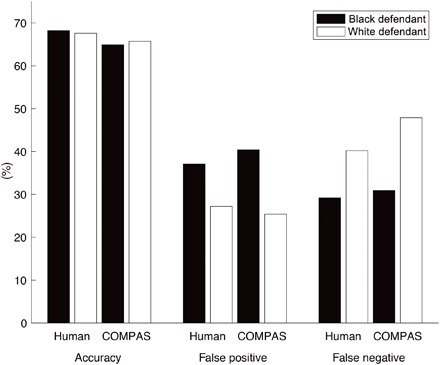
\includegraphics[width=8cm]{image1}
\caption{Die Ergebnisse der Studie [3], in der der COMPAS-Algorithmus mit zufällig gewählten Probanden bezüglich Aussagekraft der vorhergesehenen Rückfälligkeitswahrscheinlichkeit von Kriminellen verglichen wurde.\\ 
Die x-Achse beschreibt die Wahrscheinlichkeit für die auf der y-Achse beschriebenen Fälle. \\
Das erste paar Balken bezieht sich auf die Prognosen der Probanden, das zweite auf die Prognosen von COMPAS. \\
Die Farbe der Balken (schwarz oder weiß) entspricht der entsprechenden Ethnizität der Kriminellen.\\
Quelle: [3] }
\label{img1}
\end{figure}

Wenn man die Ergebnisse aus Studie [3] betrachtet (Bild \ref{img1}), springt sofort die recht große Diskrepanz zwischen weißen und Afro-Amerikanern in falschen Positiven/Negativen ins Auge: bei OCEAN ist die Rate an falschen Positiven für Afro-Amerikaner ungefähr 60\% höher als die von Weißen (ca. 40\% vs. ca. 25\%), und die Rate an falschen Negativen ungefähr 38\% niedriger (ca. 30\% vs. ca. 48\%) [3, Tabelle 1].

Diese große Differenz ist jedoch nicht nur im Algorithmus zu finden; auch die Probanden, denen die Ethnizität der Person nicht gegeben wurde, bewerteten in der Studie Afro-Amerikaner schlechter als Weiße, wenn auch nicht stark. 
Hier ist die Rate an falschen Positiven für Afro-Amerikaner ungefähr 37\% höher (ca. 37\% vs. ca. 27\%) und die an falschen Negativen ungefähr 28\% niedriger (ca. 29\% vs. ca. 40\%) [3, Tabelle 1].

Dass diese Raten dennoch schlechter in OCEAN sind impliziert, dass der Algorithmus im Durchschnitt Afro-Amerikaner strenger bewertet als Weiße. 
Dies ist problematisch, da Afro-Amerikaner ohnehin schon im Justizsystem in Amerika benachteiligt sind [4], und dieses Problem durch die Einführung von Algorithmen somit noch schlimmer werden könnte.

\FloatBarrier

% -------------------------------------------------------------------------------------------------------------------------------
\section{Mögliche Gründe für diese Resultate}
Nun muss man sich fragen, wo diese signifikante Diskrepanz an falschen Positiven/Negativen her kommen könnte - der Fragenkatalog, der von OCEAN ausgewertet wird [6] enthält nämlich keine Frage dazu, welcher Ethnizität der oder die Angeklagte angehört. 

\subsection{Die Wahrscheinlichkeit, bei einigen Fragen schlecht ab zu schneiden ist für Afro-Amerikaner höher}
Zuerst ein paar generelle Fakten über Florida, der US-Staat, in dem Broward County liegt (der Bezirk, auf den sich die Studien [1] und [3] beziehen): 
\begin{itemize} 
  \item{} Der Anteil von afro-amerikanischen Insassen in Floridas Gefängnissen höher als der von Weißen (ca. 48\% vs. ca. 40\%) [7, Seite 16]
  \item{} Die überwiegende Mehrheit der Population in Florida ist weiß (ca. 77\%) [8]. Nur ca. 17\% der Menschen in Florida ist afro-amerikanischer Ethnizität.
\end{itemize}

Daraus folgt, dass die Wahrscheinlichkeit, dass ein Elternteil oder Freund/Parter (unter der Annahme, dass Menschen einer bestimmten Ethnizität tendenziell eher Freund-/Partnerschaften mit Personen gleicher Ethnizität bilden) Zeit im Gefängnis verbracht hat, deutlich höher für Afro-Amerikaner als für Weiße ist.
Damit zeigt sich auch, warum OCEAN Afro-Amerikaner im Durchschnitt schlechter bewerten könnte: die Fragen 33 bis 36 und 38 bis 40 beziehen sich direkt darauf, ob diese jemals verhaftet wurden oder im Gefängnis waren. 

Viele weitere Fragen mit ähnlicher Begebenheit lassen sich in dem Fragebogen finden (z.B. Fragen über Gangmitgliedschaft, Probleme mit Drogen-/Alkoholbenutzung, Stabilität der Lebenssituation, Sicherheit der sozialen Umgebung oder Bildung), die Analyse dieser würde den Umfang dieses Blogeintrags jedoch sprengen.

\subsection{Die Daten, auf den die Algorithmen basieren könnten, sind rassistisch}
Unter der Annahme, dass OCEAN und ähnliche Algorithmen ihre Auswertungsweise durch Machine Learning entwickeln - eine Annahme, die momentan weder bewiesen, noch widerlegt werden kann, da wir, wie im ersten Blogeintrag erwähnt, nicht wissen, wie diese Algorithmen arbeiten - gibt es noch eine weitere Erklärung der obigen Ergebnisse: OCEAN hat "gelernt", rassistisch zu entscheiden, bzw. Attribute, die mit einer bestimmten Ethnizität korrelieren, als risikofördernd ein zu stufen.

Dies kommt daher, dass Machine Learning darauf basiert, aus gegebenen Daten einen Algorithmus zu entwickeln. D.h. benutzt man rassistisch beeinflusste Daten, wie es Rechtsprechungen sind [4], ist der daraus resultierende Algorithmus ebenfalls rassistisch.

% -------------------------------------------------------------------------------------------------------------------------------
\section{Schluss}
Zusammenfassend lässt sich sagen, dass die Einführung von Algorithmen zur Vorhersage der Rückfallswahrscheinlichkeit eines Angeklagten die in diesem Rechtssystem vorhandenen Probleme (hier Rassismus) zu amplifizieren, oder wenigstens nicht zu mindern, scheint, und diese Algorithmen dazu nicht einmal im Allgemeinen besser als Laien zu performieren scheinen.

Es wirkt nicht so, als wäre die resultierende Entlastung der Richter diese Konsequenz wert.

% -------------------------------------------------------------------------------------------------------------------------------
\section{Quellen}
\begin{itemize}
  \item{[1]}: 
    Julia Angwin, Jeff Larson, Surya Mattu, Lauren Kirchner (ProPublica): \textit{“Machine Bias”}, 2016\\
    https://www.propublica.org/article/machine-bias-risk-assessments-in-criminal-sentencing (abgerufen am 19.03.2019)

  \item{ [2]}: 
    Northpointe Inc.: \textit{"Practitioner’s Guide to COMPAS Core"}, 2015\\
    https://assets.documentcloud.org/documents/2840784/Practitioner-s-Guide-to-COMPAS-Core.pdf (abgerufen am 19.03.2019)

  \item  {[3]}:
    Julia Dressel, Hany Farid: \textit{"The accuracy, fairness, and limits of predicting recidivism"},
    Publiziert 2018 in \textit{Science Advances, Vol. 4, No. 1} \\ 
    https://www.ncbi.nlm.nih.gov/pmc/articles/PMC5777393/  (abgerufen am 19.03.2019)
  \item{[4]}:
    David S. Abrams, Marianne Bertrand, Sendhil Mullainathan: \textit{"Do Judges Vary in Their Treatment of Race?"},
    Publiziert 2012 in \textit{The Journal of Legal Studies, Vol. 41, No. 2} \\
    https://www.povertyactionlab.org/sites/default/files/publications/210\%20Do\%20Judges\%20Vary\%20Sept\%202010.pdf (abgerufen am 20.03.2019)
  \item{[5]}:
    Andrea Kienle, Gabriele Kunau: "\textit{Informatik und Gesellschaft - eine sozio-technische Perspektive"}, 2014
  \item{[6]}:
    Fragenkatalog, der von OCEAN ausgewertet wird, Northpointe Inc, 2011\\
    https://assets.documentcloud.org/documents/2702103/Sample-Risk-Assessment-COMPAS-CORE.pdf (abgerufen am 29.03.2019)
  \item{[7]}:
    Jährlicher Bericht vom Florida Department of Corrections für das Haushaltsjahr 2016 - 2017\\
    http://www.dc.state.fl.us/pub/annual/1617/FDC\_AR2016-17.pdf (abgerufen am 29.03.2019)
  \item{[8]}:
    United States Census Bureau: "\textit{Quick Facts}",
    https://www.census.gov/quickfacts/fact/table/fl/PST045218 (abgerufen am 29.03.2019)
\end{itemize}

%----------------------------------------------------------------------------------------

\end{document}
